\documentclass[9pt,letterpaper]{article}
\usepackage[margin=0.35in,top=0.28in,bottom=0.32in]{geometry}
\usepackage{amsmath,amssymb}
\usepackage{booktabs}
\usepackage{xcolor}
\usepackage{tikz}
\usetikzlibrary{arrows.meta,positioning}
\usepackage{hyperref}
\usepackage{microtype}
\usepackage{multicol}
\usepackage{titlesec}
\usepackage[T1]{fontenc}
\usepackage{lmodern}
\usepackage{colortbl}
\usepackage{fancyhdr}
\usepackage{lastpage}

% ── Colours ──
\definecolor{navy}{HTML}{1b2a4a}
\definecolor{steel}{HTML}{3d5a80}
\definecolor{tint}{HTML}{eef1f6}
\definecolor{wingreen}{HTML}{dceee2}
\definecolor{ruleblue}{HTML}{8a9ab5}
\definecolor{ltgray}{HTML}{999999}

% ── Section formatting ──
\titleformat{\section}{\bfseries\color{navy}\fontsize{8.5}{10}\selectfont}{}{0em}{}
\titlespacing{\section}{0pt}{3pt}{1pt}

% ── Page style ──
\pagestyle{fancy}
\fancyhf{}
\renewcommand{\headrulewidth}{0pt}
\renewcommand{\footrulewidth}{0.3pt}
\renewcommand{\footrule}{\hbox to\headwidth{\color{ruleblue}\leaders\hrule height \footrulewidth\hfill}\vskip 2pt}
\fancyfoot[L]{\tiny\color{ltgray} MOLLI: Model Optimization via Likelihood-based Introgression}
\fancyfoot[C]{\tiny\color{ltgray} DGX Spark (GB10, 128\,GB) $\cdot$ bfloat16 $\cdot$ 8-bit Adam}
\fancyfoot[R]{\tiny\color{ltgray} Schartl et al., \textit{Nature} (2026)}

\setlength{\parindent}{0pt}
\setlength{\parskip}{1.5pt}
\setlength{\abovedisplayskip}{2pt}
\setlength{\belowdisplayskip}{2pt}
\setlength{\columnsep}{10pt}

% ── Equation box ──
\newcommand{\eqbox}[2]{%
  \vspace{0pt}\begin{center}\colorbox{tint}{\parbox{0.95\columnwidth}{\vspace{0pt}\begin{equation}\textstyle #1\tag{#2}\end{equation}\vspace{-4pt}}}\end{center}\vspace{-2pt}}

\begin{document}

% ── TITLE ──
\begin{center}
{\fontsize{13}{15}\selectfont\bfseries\color{navy} MOLLI: Model Optimization via Likelihood-based Introgression}\\[2pt]
{\fontsize{7.5}{9}\selectfont\itshape\color{steel}
A continual learning framework for LLMs inspired by genetic introgression in \textit{Poecilia formosa} (Schartl et al., Nature 2026)}
\end{center}
\vspace{-1pt}{\color{navy}\hrule height 0.4pt}\vspace{2pt}

% ── FIGURE ──
\begin{center}
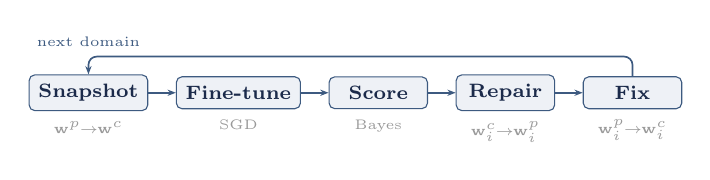
\begin{tikzpicture}[
  node distance=0.22cm and 0.35cm,
  box/.style={rectangle, rounded corners=2pt, draw=steel, fill=tint,
              minimum height=0.38cm, minimum width=1.25cm,
              font=\scriptsize\bfseries, text=navy},
  arr/.style={-{Stealth[length=3pt]}, semithick, color=steel},
  lbl/.style={font=\tiny\color{ltgray}, align=center},
]
  \node[box](s){Snapshot}; \node[box,right=of s](t){Fine-tune};
  \node[box,right=of t](sc){Score}; \node[box,right=of sc](r){Repair};
  \node[box,right=of r](f){Fix};
  \draw[arr](s)--(t); \draw[arr](t)--(sc); \draw[arr](sc)--(r); \draw[arr](r)--(f);
  % Feedback loop on top
  \draw[arr,rounded corners=3pt](f.north)--++(0,0.25)-|node[above,pos=0.5,lbl]{next domain}(s.north);
  \node[lbl,below=0.01 of s]{$\mathbf{w}^p\!\!\to\!\!\mathbf{w}^c$};
  \node[lbl,below=0.01 of t]{SGD};
  \node[lbl,below=0.01 of sc]{Bayes};
  \node[lbl,below=0.01 of r]{$\mathbf{w}^c_i\!\!\to\!\!\mathbf{w}^p_i$};
  \node[lbl,below=0.01 of f]{$\mathbf{w}^p_i\!\!\to\!\!\mathbf{w}^c_i$};
\end{tikzpicture}
\end{center}
\vspace{-4pt}
{\centering\scriptsize\color{ltgray}\textit{Figure 1.} The MOLLI evolution cycle, repeated for each new domain.\par}
\vspace{1pt}

% ── TWO COLUMNS ──
\begin{multicols}{2}

\section{1.\;The Problem}
When a language model is fine-tuned sequentially on multiple domains, each round of training overwrites weights that encoded prior knowledge. This is \textbf{catastrophic forgetting}. LoRA reduces this by training small adapter matrices, but each adapter merge dilutes prior adaptations: after $N$ merges, each domain retains roughly $1/N$ of its contribution (the \textbf{O(1/N) dilution problem}). No existing method can identify \emph{which specific weight groups} were damaged by new training, or selectively undo that damage.

\section{2.\;Biological Inspiration}
The Amazon Molly (\textit{P.~formosa}) reproduces asexually yet has thrived for ${\sim}100{,}000$ years, defying the prediction that without sexual recombination, harmful mutations accumulate irreversibly until extinction (Muller's Ratchet). A 2026 Nature paper revealed the mechanism: \textbf{gene conversion}---a repair process where the organism's two chromosome copies compare themselves, and when one carries a harmful mutation, the healthy copy overwrites it. MOLLI applies this principle to neural networks. The model's weights are the genome. Fine-tuning introduces ``mutations.'' A quantized checkpoint serves as the healthy reference. And a Bayesian scoring system plays the role of natural selection, deciding which changes to keep and which to repair.

\section{3.\;Method}

\textbf{Dual-strand encoding.}
We partition model parameters into $L$ functional groups called \textbf{genes}---each attention head, MLP block, and LayerNorm is one gene ($L\!=\!928$ for 7B parameters). Two copies are maintained: the \textbf{primary} $\mathbf{w}^p$ (live trainable weights) and the \textbf{complement} $\mathbf{w}^c$ (int16-quantized snapshot from before training). Overhead: 2 bytes/parameter.

\textbf{Gene scoring.}
After fine-tuning, we estimate the effect of reverting each gene $i$ on the loss $\mathcal{L}_j$ of prior domain $j$. The partial derivative of the loss with respect to each parameter tells us how sensitive the loss is to that parameter; the complement--primary difference tells us how much it changed. Summing their element-wise product over all parameters in a gene gives the estimated reversion effect:

\eqbox{\delta_{ij} = \!\sum_{k \in g_i}\! \tfrac{\partial \mathcal{L}_j}{\partial \theta_k} \!\cdot\! \bigl(w^c_k - w^p_k\bigr)}{1}

where $g_i$ is the set of parameter indices belonging to gene $i$. This is a first-order Taylor approximation. One forward+backward pass yields all partial derivatives, from which all $L\!=\!928$ gene scores are extracted by slicing. Cost: $\mathcal{O}(N_\text{obj})$, not $\mathcal{O}(L \!\times\! N_\text{obj})$.

\textbf{Why raw scores aren't enough.}
The score $\delta_{ij}$ depends on which evaluation samples we used---it is a noisy estimate. A gene might appear damaged purely by statistical fluctuation. Repairing based on noisy scores would introduce unnecessary changes. We need to separate genuine signal from noise.

\textbf{Bayesian shrinkage.}
We apply \textbf{empirical Bayes} to obtain calibrated probabilities. We split evaluation data in half, score each half independently, and measure agreement (split-half correlation $r$). High agreement ($r \approx 1$) means the scores are reliable; low agreement means noise dominates. We decompose observed variance into signal $\tau^2$ and noise $\sigma^2$, then compute a shrinkage factor:

\eqbox{\tau^2 = \max\!\bigl(0,\,\textrm{Var}(\delta) - \sigma^2\bigr),\;\; B = \tfrac{\tau^2}{\tau^2 + \sigma^2},\;\; \delta^*_{ij} = B\delta_{ij} + (1\!-\!B)\mu_0}{2}

When $B \approx 1$, data has high signal-to-noise and we trust observed scores. When $B \approx 0$, noise overwhelms signal and scores are shrunk toward the mean $\mu_0$ (assuming the gene is unaffected). This prevents false-positive repairs. In our experiments, $B$ ranged from 0.75 (SNR\,=\,3.1) to 0.999 (SNR\,=\,842.5), with split-half $r = 0.83$--$0.999$.

\textbf{Repair decision.}
From the shrunk scores, we compute the posterior probability that gene $i$ is deleterious to domain $j$:

\eqbox{P(\textrm{del}_{ij}) = 1 - \Phi\!\bigl(\tfrac{-\delta^*_{ij}}{\sqrt{V_\textrm{post}}}\bigr)}{3}

Repair gene $i$ if $\max_j P(\textrm{del}_{ij}) - \alpha\, P(\textrm{ben}_i) > \theta$,

where $\Phi$ is the normal CDF, $\alpha$ balances prior-domain protection against current-domain benefit, and $\theta$ is the repair threshold. Repair copies $\mathbf{w}^c_i \!\to\! \mathbf{w}^p_i$, reverting that gene. Capped at 15\% of genes per cycle. Genes with $P(\textrm{del}) < 0.3$ on all priors are \textbf{fixed} ($\mathbf{w}^p_i \!\to\! \mathbf{w}^c_i$), permanently accepting the change.

\section{4.\;Results}
Qwen2.5-7B (928 genes), 100 train / 49 eval $\times$ 256 tokens, 3 epochs, bfloat16, 8-bit Adam.

\vspace{2pt}
\resizebox{\columnwidth}{!}{%
\begin{tabular}{@{}lcccc@{}}
\toprule
\textbf{Domains} & \textbf{MOLLI} & \textbf{LoRA} & $\boldsymbol{\Delta}$ & \textbf{Time (M/L)} \\
\midrule
3 (code$\to$legal$\to$med) & \textbf{1.60} & 2.10 & $-$24\% & 38/15\,m \\
\rowcolor{wingreen}
5 (+ science, finance) & \textbf{1.11} & 1.45 & $-$23\% & 113/49\,m \\
6 (+ general) & \textbf{1.52} & 1.60 & $-$5\% & 146/62\,m \\
\bottomrule
\end{tabular}}
\vspace{1pt}
{\centering\scriptsize\color{ltgray}\textit{Table 1.} GM perplexity (lower = better). Best: 1.11 at 5 domains.\par}
\vspace{2pt}

\resizebox{\columnwidth}{!}{%
\begin{tabular}{@{}lccccccc@{}}
\toprule
& gen & code & leg & med & sci & fin & \textbf{GM} \\
\midrule
\rowcolor{wingreen}
\textbf{MOLLI\,5d} & 1.06 & 1.25 & 1.10 & 1.14 & 1.06 & 1.06 & \textbf{1.11} \\
LoRA\,5d & 1.10 & 1.63 & 1.83 & 2.29 & 1.10 & 1.10 & 1.45 \\
\midrule
\textbf{MOLLI\,6d} & 1.05 & 1.53 & 2.53 & 2.80 & 1.05 & 1.05 & \textbf{1.52} \\
LoRA\,6d & 1.11 & 1.68 & 2.81 & 2.65 & 1.11 & 1.11 & 1.60 \\
\bottomrule
\end{tabular}}
\vspace{1pt}
{\centering\scriptsize\color{ltgray}\textit{Table 2.} Per-domain PPL. At 5d, MOLLI retains all domains $\leq$ 1.25.\par}
\vspace{2pt}

\textbf{Findings.}
MOLLI achieves 23--24\% lower GM PPL at 3 and 5 domains. At 5d, all priors $\leq$1.25; LoRA degrades to 2.29/1.83. At 6d, the gap narrows (15\% repair cap bottleneck). 139/928 genes repaired per cycle---targeted, selective intervention.

\end{multicols}

\end{document}
